\documentclass[a4paper,halfparskip,11pt,twoside]{scrartcl}
\usepackage{schlaue_schwaerme}

\usepackage{url}

\newcommand{\R}{\mathbb{R}}
\newcommand{\cupdot}{\ensuremath{\mathaccent\cdot\cup}} % disjuncted union

\begin{document}
\init{}

\pgMaketitle{User's Guide}{
\begin{pgArrowitemize}
	\item Alexander Klaas
	\item Andreas Cord-Landwehr
	\item Christoph Raupach
	\item Christoph Weddemann
	\item Daniel Warner
	\item Daniel Wonisch
	\item Kamil Swierkot
	\item Marcus Märtens
	\item Martina Hüllmann
	\item Peter Kling
	\item Sven Kurras
\end{pgArrowitemize}
}

\section{Introduction}
This document shall help you to use the \RSS\ to simulate robot swarms and to get useful information by the visualization and statistics modules.

For this purpose the document is divided in several sections. It will be usefull if you just start with the ``Getting Started!'' section and play a little bit with the simulator and continue with reading the more detailed information on input parameters, input-file specifications, generating simulations and getting statistics.


\section{Getting Started}
For a first test of \RSS you can simply run it in generation mode, and use the generated scenario with one of our default algorithms. All example files can be found in subdirectory {\tt ProjectFiles} of the install directory. Here we will present a short example how to simulate the behavior of the {\sc CenterOfGravity} algorithm (COG).

\begin{enumerate}
	\item Change to the directory that contains the \RSS binary.
	\item Run the following command:

		\centerline{\tt RobotSwarmSimulator -{}-generate -{}-distr-pos 20 -{}-algorithm COGRobot}

		This will generate a simulation specification in form of the following files:
		\begin{itemize}
			\item {\tt newrandom.swarm} -- contains information about the simulation process
			\item {\tt newrandom.robot} -- contains information about the robots
			\item {\tt newrandom.obstacle} -- contains information about the obstacles
		\end{itemize}
		The last two files are referenced in the {\tt .swarm} file. Thus, to load the simulation, you only need to load the {\tt .swarm} file. Note that all these files
are simple text files that can be edited by hand.
	\item Run the command:

		\centerline{\tt RobotSwarmSimulator -{}-project-file newrandom -{}-output mylogs}

		This will start the simulation process. There are various keyboard shortcuts that can be used to control the simulation. Press \fbox{\tt h} for an overview. You can quit the simulation by pressing \fbox{\tt q}.
	\item The previous step will generate various output files in the subdirectory {\tt mylogs}, mainly produced by the statistics module of the \RSS. You may directly use Gnuplot to analyze these files.
\end{enumerate}
This simple example can be used as base for further test runs. Please look at the following chapters to get specifications of the input--files and the user's inferface.

\section{Running the \RSS\ with Parameters}
The \RSS\ exists as executable for Linux, Mac OS X and Windows. Each execution of the \RSS\ needs specific parameters that are mandatory. By running the \RSS\ you have to specify at least, which kind of execution you want. There are two main options:

\begin{itemize}
 \item By adding the parameter {\tt -{}-generate} the generation mode is started to create new input--files. This will generate three different files having the suffixes {\tt .swarm}, {\tt .robot} and {\tt .obstacle}. The most important of these is the {\tt .swarm} file, which references the other two files.
\item Using the parameter {\tt -{}-project-file $\langle$your\_input\_file$\rangle$}, the common simulation mode is started. In this case, <your input file> should be the name of a file having the suffix {\tt .swarm} (e.g. generated with generation mode).
\end{itemize}

There other command line options that may be used to show help or about messages and to customize the generation or simulation mode. Start the \RSS with the parameter {\tt -{}-help} to get an overview. A typical session may look like this:

\begin{verbatim}
    ./RobotSwarmSimulator --help
    ./RobotSwarmSimulator --project-file <path_to_testdata>/testfile_2 \\
                          --output <path_to_output_files> \\
                          --history-length 10
\end{verbatim}

All of the options listed in Listing~\ref{lst:RSS-help} can be used. Further information for this parameters can be found in the following sections. The definition of most of the parameters can be found in Table~\ref{tab:mainvars}.

\begin{lstlisting}[caption={RSS Helpline},label=lst:RSS-help]
localhost:~$ ./RobotSwarmSimulator --help

General options:
 --help                shows this help message
 --version             shows version of RobotSwarmSimulator
 --about               tells you who developed this awesome piece of software

Generator options:
 --generate                      switch to generator mode
 --seed arg (=1)                 seed for random number generator
 --robots arg (=100)             number of robots
 --algorithm arg (=NONE)         name of algorithm or lua-file
 --worldfile arg (=newrandom)    world-file for output
 --robotfile arg (=newrandom)    robot-file for output
 --obstaclefile arg (=newrandom) obstacle-file for output
 --add-pos-handler               add position request handler for testing
 --add-vel-handler               add velocity request handler for testing
 --add-acc-handler               add acceleration request handler for testing
 --distr-pos arg (=0)            distribute position in cube [0;distr-pos]^3
 --min-vel arg (=0)              distribute velocity in sphere with radius
                                 min-vel
 --max-vel arg (=0)              distribute velocity in sphere with max-vel
 --min-acc arg (=0)              distribute acceleration in sphere with radius
                                 min-acc
 --max-acc arg (=0)              distribute acceleration in sphere with radius
                                 max-acc
 --distr-coord                   distribute robot coordinate-systems uniformly

Simulation options:
 --project-file arg         Project file to load
 --output arg               Path to directory for output
 --history-length arg (=25) history length
\end{lstlisting}


\subsection{General options}
\begin{description}
	\item [-{}-help] Lists all possible options including a short description.
	\item [-{}-version] This option shows the version information of your \RSS.
	\item [-{}-about] Get information about the developer team, contact information and more.
\end{description}

\subsection{Generator options}
\begin{description}
	\item [-{}-generate] Switch to generator mode. This is necessary for the further options of this section.
	\item [-{}-seed arg] Sets the seed for the random number generator for robot generation. If not set the seed is {\tt 1}. An unsigned integer value is expected.
	\item [-{}-robots arg] The number of robots to be generated. The default number is 100. An unsigned integer value is expected.
	\item [-{}-algorithm arg] The name of the algorithm the robots should use. If not set the algorithm {\tt SimpleRobot} is used. This is only a stub without any functionality. Also the name of a lua-file can be given. Extensionsion {\tt .lua} is mandatory for lua-files.
	\item [-{}-worldfile arg] The name of the worldfile that shall be generated. Default is {\tt newrandom}. File-name without extension is expected.
	\item [-{}robotfile arg] The name of the robotfile that shall be generated. Default is {\tt newrandom}. File-name without extension is expected.
	\item [-{}-obstaclefile arg] The name of the obstaclefile that shall be generated. Default is {\tt newrandom}. File-name without extension is expected.
	\item [-{}-add-pos-handler] Causes the generated files to contain a position request handler with reasonable default values. If you need a more sophisticated position request handler, you have to edit the generated {\tt .swarm} file yourself.
	\item [-{}-add-vel-handler] Causes the generated files to contain a velocity request handler with reasonable default values. If you need a more sophisticated velocity request handler, you have to edit the generated {\tt .swarm} file yourself.
	\item [-{}-add-acc-handler] Causes the generated files to contain a acceleration request handler with reasonable default values. If you need a more acceleration request handler, you have to edit the generated {\tt .swarm} file yourself.
	\item [-{}-distr-pos arg] Distributes the position of robots uniformly at random in the cube $[-arg/2,+arg/2]^3$
 If not set, all robots are at position zero.
	\item [-{}-min-vel arg] The robots will be generated with a velocity distributed uniformly between the given minimum and maximum velocity (see {\tt -{}---max-vel}). This parameter defaults to 0.
	\item [-{}-max-vel arg] The robots will be generated with a velocity distributed uniformly between the given minimum and maximum velocity (see {\tt -{}---min-vel}). This parameter defaults to 0.
	\item [-{}-min-acc arg] The robots will be generated with a acceleration distributed uniformly between the given minimum and maximum velocity (see {\tt -{}---max-acc}). This parameter defaults to 0.
	\item [-{}-max-acc arg] The robots will be generated with a acceleration distributed uniformly between the given minimum and maximum velocity (see {\tt -{}---min-acc}). This parameter defaults to 0.
	\item [-{}-distr-coord arg] Generates uniformly distributed coordinate--systems for the robots. If this option is not given, all robots will have the same global coordinate system (defined by a unit matrix).
 If not set, all velocities are zero.
\end{description}

\subsection{Simulation options}
\begin{description}
	\item [-{}-project-file arg] Specifies the project file use. Use this parameter to load a simulation specified by a {\tt .swarm} file. Not that you may ommit the file extension {\tt .swarm}. Mandatory for simulation.
	\item [-{}-output arg] Specifies a directory to be used for files generated by the simulation (e.g. statistics files for Gnuplot). The given name is interpreted relative to the current directory and will create the directory if necessary. If ommitted, all generated files will be stored in the current directory.
	\item [-{}-history-length arg] Sets the history length i.e. the length of the ringbuffer that stores past simulation states. Standard is 25 (which should be a good choice in most cases). An unsigned integer is expected.
\end{description}


\section{Using the Simulator-Interface}
During the simulation it is possible to interact with the simulation in different ways. The following hot-keys are supported while simulation:

\begin{description}
	\item [\fbox{\tt Space}] Start/Stop
	\item [\fbox{\tt Q}] the Quit \RSS\
	\item [\fbox{\tt F1}] Help
	\item [\fbox{\tt G}] Show Center of all gravity of Swarm
	\item [\fbox{\tt V}] Show velocity vectors
	\item [\fbox{\tt B}] Show acceleration vectors
	\item [\fbox{\tt K}] Show global coordinates system
	\item [\fbox{\tt W},\fbox{\tt A},\fbox{\tt S},\fbox{\tt D}] In the corresponding camera mode use \fbox{\tt W} for up  and \fbox{\tt S} for down %TODO what about a,d?
	\item [Arrow-Keys] left, right, before, behind
	\item [Mouse] Mouse for spinning
	\item [\fbox{\tt +}, \fbox{\tt -}] increase/ decrease simulation-speed by constant
	\item [\fbox{\tt *},\fbox{\tt /}] double/ half simulation-speed
	\item [\fbox{\tt C}] Change camera
\end{description}
%TODO(cola) compare with final version

\section{Robot Definitions by LUA-files}
There are two ways to define a new robot. One way is hardcoded in the \RSS\, the other way is to define the robots by scripting their behavior in the {\sffamily Lua} scripting language. For example Listing~\ref{lst:cog-lua} shows you how to formulate the COG-algorithm in Lua.

\todo{yeah, how can I do this?}

\lstset{language=c}
\begin{lstlisting}[caption={COG algorithm in Lua},label=lst:cog-lua]
function main() 
    robots = get_visible_robots();
    center = get_position(get_own_identifier());
    for i = 1, #robots do
        center = center + get_position(robots[i]);
    end
    center = center / (#robots+1);
    add_position_request(center);
end
\end{lstlisting}

\section{Statistics}
A simulation run results in three output files of statistics:

\begin{itemize}
\item \texttt{gnuplot\_20091224\_184129\_ALL.plt} (GNUPlot-configuration file)
\item \texttt{output\_20091224\_184129\_ALL.plt} (according statistic data)
\item \texttt{output\_20091224\_184129\_DATADUMP\_FULL.plt} (complete data dump)
\end{itemize}

The file-names results from current date (year, month, day), the current time (hour, minute, second), followed by description of screened object subset (e.\.g. \texttt{ALL, MASTERS,}\dots). For each entry in STATISTICS\_SUBSETS there will be created one such data pair.

\newpage
\appendix

\section{Visualization with GNUPlot}

\paragraph{Anzeige mit GNUPlot}
Zur Anzeige der Statistiken eines abgeschlossenen Simulationsdurchlaufes muss die entsprechende GNUPlot-Konfigurationsdatei mit GNUPlot geöffnet werden: Unter Unix-System kann man hierfür nach Aufruf von \texttt{\$ gnuplot} die interaktive GNUPlot-Shell verwenden (\texttt{> load ``gnuplotfile.plt``}). Weitere Befehle mit \texttt{> help}. Alternativ kann man sich die Ausgabe direkt anzeigen lassen mittels Shellkommando \texttt{\$ gnuplot -persist ''gnuplotfile.plt``}, wobei das \texttt{-persist} bewirkt, dass das Anzeigefenster auch nach Erstellen der Ausgabe geöffnet bleibt. Weitere Flags siehe \texttt{\$ man gnuplot}.


\paragraph{Konfiguration der Anzeige}
Der Inhalt der Datei \texttt{output\_20091224\_184129\_ALL.plt} könnte auszugsweise so aussehen:

\begin{center}
\texttt{\begin{tabular}{rrrl}
\# time & avg\_spd & minball\_x & (...) \\
\hline
0 & 9.2 & 20.5 \\
1 & 11.3 & 21.5 \\
4 & 9.1 & 21.9 \\
6 & 7.5 & 22.3
\end{tabular}}
\end{center}

Jede Zeile enthält die statistischen Daten zu einem bestimmten Zeitpunkt. Der Beginn einer neuen Spalte wird hierbei durch (mindestens) ein Leerzeichen gekennzeichnet. '\#' leitet eine Kommentarzeile ein.

In der Datei \texttt{gnuplot\_20091224\_184129\_ALL.plt} findet nun die Formatierung der Daten für die Anzeige statt und kann beliebig geändert werden:

\begin{verbatim}
# statistics of the simulation
#====================================
set title ' SCHLAUE SCHWÄRME '
set xrange []
set yrange []
set grid
set pointsize 0.5
set xlabel 'time'
set ylabel ''
plot 'output_(...)_ALL.plt' using 1:2 title 'avg_spd' with linespoints, \
     'output_(...)_ALL.plt' using 1:3 title 'minball_x' with linespoints
\end{verbatim}

Die Angaben haben folgende Bedeutung:
\begin{itemize}
\item \texttt{set title '\textit{Titel}'} erzeugt einen zentrierten Titel am oberen Teil der grafischen Darstellung.
\item \texttt{set xrange [\textit{min}:\textit{max}]} begrenzt den horizontal sichtbaren Bereich zwischen den Werten \texttt{\textit{min}} und \texttt{\textit{max}}, \texttt{set xrange []} führt diese Skalierung auf Grundlage der vorliegenden Daten automatisch durch.
\item \texttt{set grid} blendet ein Gitternetz ein.
\item \texttt{set pointsize \textit{multiplikator}} skaliert die Größe der Punkte (falls eine Darstellung gewählt wird, welche Punkte beinhaltet) gemäß \texttt{\textit{multiplikator}}.
\item \texttt{xlabel '\textit{Label}'} beschriftet die X-Achse.
\end{itemize}
Diese Angaben beinhalten also \textit{nur} grafische grafische Aspekte, die z.B. für die Verwendung in Dokumentationen angepasst werden können. Die Einstellungen der anzuzeigenden Daten finden erst daraufhin statt:

\begin{itemize}
 \item \texttt{plot '\textit{Dateiname.plt}'} leitet den tatsächlichen Vorgang der Darstellung ein. Hierbei werden die Daten aus der angegebenen Datei gelesen. Durch \texttt{using 1:2} werden die erste und die zweite Spalte gegeneinander dargestellt, wobei der erstgenannte Spaltenindex, also \texttt{time}, die X-Koordinate und folglich \texttt{avg\_spd} die Y-Koordinate definiert. \texttt{title `avg\_speed'} fügt für die definierte Funktion einen Legendeneintrag mit dem Titel \texttt{avg\_speed} hinzu. Der Zusatz \texttt{with linespoints} beschreibt die Darstellung durch mit Linien verbundene Zeichen an den Datenpunkten. \texttt{linespoints} kann auch ersetzt werden durch:
\begin{itemize}
\item \texttt{lines} verbindet jeden Datenpunkt mit einer Linie
\item \texttt{dots} zeigt einzelne Punkte an (sinnvoll bei vielen Datenpunkten)
\item \texttt{points} fügt ein Zeichen an der Position des Datenpunktes ein. Die Größe kann durch den Befehl \texttt{set pointsize} geändert werden
\item \texttt{linespoints} erstellt gleichzeitig \textit{points} und \textit{lines}
\item \texttt{impulses} erzeugt eine vertikale Linie ausgehend von der X-Achse zum Datenpunkt
\end{itemize}
Zum Plotten einer weiteren Funktion in derselben Darstellung wird die gleiche Struktur durch ein Komma getrennt angehangen (auch aus verschiedenen Quelldateien). Dies ermöglicht auf einfache Art, dass die Darstellung der Statistiken unterschiedlicher Simulationsdurchläufe in einer Grafik dargestellt werden können.
\end{itemize}

\paragraph{Ergebnis}~\\

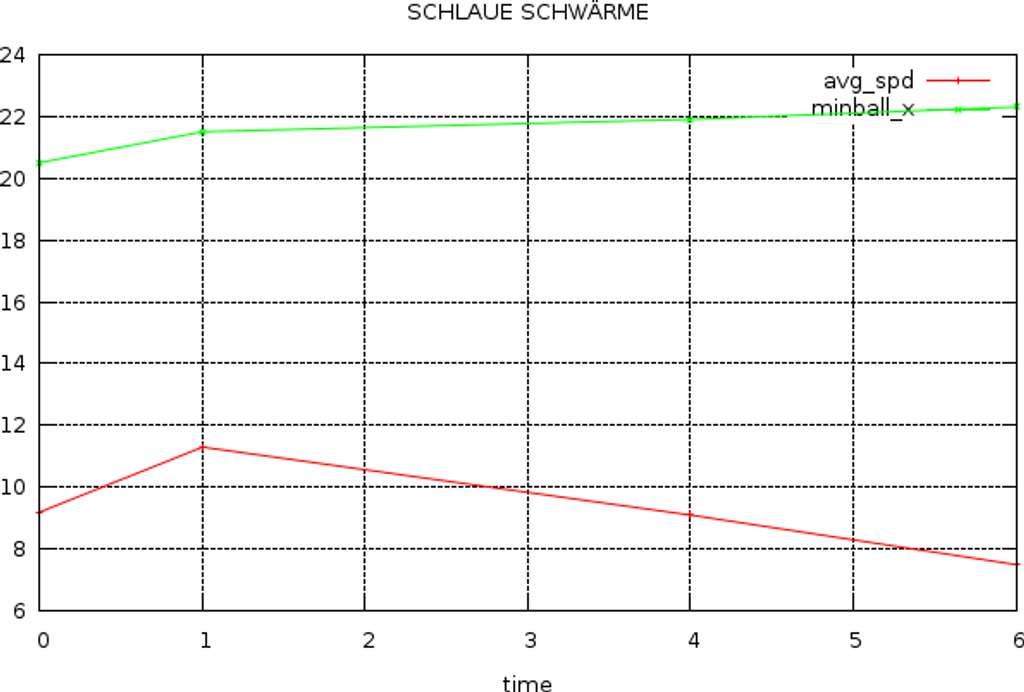
\includegraphics[width=\textwidth]{stats-howto-gnuplot.png}

\paragraph{Weitere Informationen zu GNUPlot}~\\

\begin{tabular}{l}
 $[1]$ offizielle Homepage: \url{http://www.gnuplot.info/} \\
 $[2]$ Grundkurs: \url{http://userpage.fu-berlin.de/~voelker/gnuplotkurs/gnuplotkurs.html}
\end{tabular}
	\newpage
%%
% This file is part of the User's Guide to RSS
% It contains the appendix for inputfile specifications
%%

\section{Input-file Specifications}

There are exactly four kinds of input files for the \RSS. This includes the project specification files and also the \Lua-script-files that define the robot behaviour.
\begin{enumerate}
	\item The main projectfile containing information about the model. The extension of this type of file is "`.swarm"'.
	\item A file containing robot information. The extension of this file is "`.robot"'.
	\item A file containing obstacle information. The extension of this file is "`.obstacle"'.
	\item \Lua\ file that describes the robot behavouir. The extension of this file is "`.lua"'.
\end{enumerate}


\subsection{Main projectfile}
The following specifications hold only for the main projectfile (with extension \texttt{.swarm}):
\begin{itemize}
	\item A comment begins with a '\#'.
	\item A line is a comment line (beginning with a '\#'), an empty line or a line containing a variable followed by an equal sign followed by a \emph{quoted} value of this variable. Example:
	\begin{verbatim}
		VAR_1="value"
		VAR_2 = "value"
		VAR_3= "value"
		VAR_4 ="value"
	\end{verbatim}
	\item a variable name has to be of the following form: \texttt{[A-Z0-9\_]$^+$}
\end{itemize}


\subsubsection{Variables}
The main project file contains the variables defined in Tables \ref{tab:mainvars} and \ref{tab:mainvars2}.
	
Also the following should be considered:
\begin{itemize}
	\item The order of the variables in the main project file is not important.
	\item If a variable does not appear in the main projectfile, then its default value will be used if such a default value does exist (otherwise an exception will be thrown while loading the main project-file).
\end{itemize}

\clearpage
\begin{sidewaystable}
\scriptsize
	\begin{tabular}{|l|p{0.3\textwidth}|p{0.3\textwidth}|p{0.2\textwidth}|}
		\hline
		\textbf{Variable name} & \textbf{Possible Values} & \textbf{Description} & \textbf{Default}\\\hline\hline
		\texttt{PROJECT\_NAME} & String & Name of the project & -- \\\hline
% 		\texttt{BATTLEBOX\_SIZE} & width, for instance 100 denotes a box of size $100\times 100\times 100$ & Size of bounding box of initial robot positions\\\hline
		\texttt{COMPASS\_MODEL} & Still needs to be specified by the ASG-Team. For instance \texttt{NO\_COMPASS} & Compass model & FULL\_COMPASS\\\hline
		\texttt{ROBOT\_FILENAME} & For instance \texttt{robot\_file}. The extension of the file must not be appended in this variable. & Filename of the robotfile & same as project file\\\hline
		\texttt{OBSTACLE\_FILENAME} & For instance \texttt{obstacle\_file}.  The extension of the file must not be appended in this variable. & Filename of the robotfile & same as project file\\\hline
		\texttt{STATISTICS\_SUBSETS} & A concatenation of none or more of the following strings: \{ALL\}, \{ACTALL\}, \{INACTALL\}, \{MASTERS\}, \{ACTMASTERS\}, \{INACTMASTERS\},  \{SLAVES\}, \{ACTSLAVES\}, \{INACTSLAVES\} &  Defines the subsets of all robots for which to calculate individual statistical data. E.\,g. ``\{ALL\} \{MASTERS\}'' will produce statistical information on \textit{all} robots as well as on \textit{masters only} & NONE\\\hline
		\texttt{STATISTICS\_TEMPLATE} & One of the following: ``ALL'', ``BASIC'' or ``NONE'' & Identifies the set of informations to calculate for each subset. & ALL\\\hline
		\texttt{STATISTICS\_DATADUMP} & Either ``FULL'' or ``NONE'' & Whether or not detailled information (E.\,g. all robots positions at each event) should be streamed to a file during simulation. & NONE\\\hline
		\texttt{ASG} & \texttt{SYNCHRONOUS}, \texttt{ASYNCHRONOUS} or \texttt{SEMISYNCHRONOUS} & Type of ASG & \texttt{SYNCHRONOUS}\\\hline
		  \texttt{ASYNC\_ASG\_SEED} & unsigned int & Seed for asynchronous ASG, only set if ASG=ASYNCHRONOUS & - \\\hline
		    \texttt{ASYNC\_ASG\_PART\_P} & double & Participation Probability for asynch ASG, only set if ASG = ASYNCHRONOUS & - \\\hline
		 \texttt{ASYNC\_ASG\_TIME\_P} & double & parameter governing the timing of asynch ASG, only set if ASG = ASYNCHRNOUS. The lower this is the more often events happen. & - \\\hline
		 
		\texttt{ROBOT\_CONTROL} &  see section \ref{sec:robotControl} & RobotControl to use & -\\\hline
		\texttt{CAMERA\_POSITION} &  \texttt{x,y,z}, where $x,y,z\in\mathbb{R}$& Initial camera position & \texttt{0,0,0}\\\hline
		\texttt{CAMERA\_DIRECTION} &  \texttt{x,y,z}, where $x,y,z\in\mathbb{R}$& Initial camera direction & \texttt{1,0,0}\\\hline


		 
	\end{tabular}
	\caption{Variables in the main project file}\label{tab:mainvars}
\end{sidewaystable}
\thispagestyle{empty}
\clearpage

\clearpage
\begin{sidewaystable}
\scriptsize
	\begin{tabular}{|l|p{0.3\textwidth}|p{0.3\textwidth}|p{0.1\textwidth}|}
		\hline
		\textbf{Variable name} & \textbf{Possible Values} & \textbf{Description} & \textbf{Default}\\\hline\hline

		 \texttt{MARKER\_REQUEST\_HANDLER\_TYPE} &  element from $\{$\texttt{STANDARD,NONE}$\}$ & Type of Marker Request Handler to use & $\{$\texttt{NONE}$\}$\\\hline
		 
		\texttt{TYPE\_CHANGE\_REQUEST\_HANDLER\_TYPE} &  element from $\{$\texttt{STANDARD,NONE}$\}$ & Type of Type Change Request Handler to use. & $\{$\texttt{NONE}$\}$\\\hline
		
		\texttt{POSITION\_REQUEST\_HANDLER\_TYPE} &  element from $\{$\texttt{VECTOR,NONE}$\}$ & Type of Position Request Handler to use & $\{$\texttt{NONE}$\}$\\\hline

		\texttt{VELOCITY\_REQUEST\_HANDLER\_TYPE} &  element from $\{$\texttt{VECTOR,NONE}$\}$ & Type of Velocity Request Handler to use & $\{$\texttt{NONE}$\}$\\\hline

		\texttt{ACCELERATION\_REQUEST\_HANDLER\_TYPE} &  element from $\{$\texttt{VECTOR,NONE}$\}$ & Type of Acceleration Request Handler to use & v\\\hline
		
		 \texttt{STANDARD\_MARKER\_REQUEST\_HANDLER\_SEED} &  integer & Seed for Marker Request Handler to use & $\{$\texttt{NONE}$\}$\\\hline
		 
		\texttt{STANDARD\_TYPE\_CHANGE\_REQUEST\_HANDLER\_SEED} &   integer & Seed for Type Change Request Handler to use. & -\\\hline
		
		\texttt{POSITION\_REQUEST\_HANDLER\_SEED} &   integer & Seed for Position Request Handler to use & -\\\hline

		\texttt{VELOCITY\_REQUEST\_HANDLER\_SEED} &   integer & Seed for Velocity Request Handler to use & -\\\hline

		\texttt{ACCELERATION\_REQUEST\_HANDLER\_SEED} &   integer & Seed for Acceleration Request Handler to use & -\\\hline
		
		
		
		 \texttt{STANDARD\_MARKER\_REQUEST\_HANDLER\_DISCARD\_PROB} &  element from interval $[0,1]$ & Discard probability for Marker Request Handler to use & -\\\hline
		 
		\texttt{STANDARD\_TYPE\_CHANGE\_REQUEST\_HANDLER\_DISCARD\_PROB} & element from interval $[0,1]$ & Discard probability  for Type Change Request Handler to use. & -\\\hline
		
		\texttt{POSITION\_REQUEST\_HANDLER\_DISCARD\_PROB} & element from interval $[0,1]$ & Discard probability  for Position Request Handler to use & -\\\hline

		\texttt{VELOCITY\_REQUEST\_HANDLER\_DISCARD\_PROB} & element from interval $[0,1]$ & Discard probability  for Velocity Request Handler to use & -\\\hline

		\texttt{ACCELERATION\_REQUEST\_HANDLER\_DISCARD\_PROB} & element from interval $[0,1]$ & Discard probability  for Acceleration Request Handler to use & -\\\hline
		
		
		\texttt{POSITION\_REQUEST\_HANDLER\_MODIFIER} & list of vector modifiers (see \ref{sec:vectorModifiers}) & List of vector modifiers for Position Request Handler to use & -\\\hline

		\texttt{VELOCITY\_REQUEST\_HANDLER\_MODIFIER} & list of vector modifiers (see \ref{sec:vectorModifiers}) & List of vector modifiers for Velocity Request Handler to use & -\\\hline

		\texttt{ACCELERATION\_REQUEST\_HANDLER\_MODIFIER} & list of vector modifiers (see \ref{sec:vectorModifiers}) & List of vector modifiers for Acceleration Request Handler to use & -\\\hline		
				
	\end{tabular}
	\caption{Variables in the main project file}\label{tab:mainvars2}
\end{sidewaystable}
\enlargethispage*{2cm}
\thispagestyle{empty}
\clearpage

\subsubsection{Activation Sequence Generators}

There are two Activation Sequence Generators (ASGs). A synchronous ASG and an asynchronous ASG.

To use the synchronous ASG one only needs to set the variable \texttt{ASG}=\texttt{SYNCHRONOUS}. No further variables need to be set.
To use the asynchronous ASG one needs to set \texttt{ASG}=\texttt{ASYNCHRONOUS}. Furthermore one needs to set the following variables:
\begin{itemize}
\item \texttt{ASYNC\_ASG\_SEED}: Seed for the ASG
\item \texttt{ASYNC\_ASG\_PART\_P}: The higher this is, the more robots are activated for each event. Goes from 0.0 to 1.0.
\item \texttt{ASYNC\_ASG\_TIME\_P}: The lower this is the smaller is the time difference between events. Be careful with very high values as buffer overflows might happen. Goes from 0.0 to 1.0.
\end{itemize}

\subsubsection{Vector Modifiers}\label{sec:vectorModifiers}

The list of vector modifiers is a (not necessarily nonempty) list, i.\,e. 
\begin{center}\scriptsize
	\texttt{(VECTOR\_MODIFIER\_1);(VECTOR\_MODIFIER\_2);...}
\end{center}
The order of the elements of this list is important. If no Vector Modifier shall be used for the corresponding Request Handler, then use \texttt{VECTOR\_MODIFIERS=}''''.

An element \texttt{VECTOR\_MODIFIER\_k} of the Vector Modifier list is a tuple, defined as follows:
\begin{center}\scriptsize
	\texttt{VECTOR\_MODIFIER\_k=(VECTOR\_MODIFIER\_TYPE,VECTOR\_MODIFIER\_PARAM\_1,VECTOR\_MODIFIER\_PARAM\_2,..)}
\end{center}
The number and types of paramters like \texttt{VECTOR\_MODIFIER\_PARAM\_1,\newline VECTOR\_MODIFIER\_PARAM\_2,\dots} depends on the corresponding type of the Vector Modifier. Currently there are the following types of Vector Modifiers:
\begin{itemize}
	\item VectorDifferenceTrimmer
	\item VectorTrimmer
	\item VectorRandomizer
\end{itemize}
I.\,e. the value of \texttt{VECTOR\_MODIFIER\_TYPE} needs to be \texttt{VECTOR\_DIFFERENCE\_TRIMMER, VECTOR\_TRIMMER} or \texttt{VECTOR\_RANDOMIZER}.

\paragraph{VectorDifferenceTrimmmer} If \texttt{VECTOR\_MODIFIER\_TYPE} is equal to\newline \texttt{VECTOR\_DIFFERENCE\_TRIMMER}, then the following parameters are expected:
\begin{enumerate}
	\item length of type double
\end{enumerate}
I.\,e. an element of the \texttt{VECTOR\_MODIFIERS}-list of type \texttt{VECTOR\_DIFFERENCE\_TRIMMER} may look like: \texttt{(VECTOR\_DIFFERENCE\_TRIMMER,5.2)}.

\paragraph{VectorTrimmer} If vector modifier type equals \texttt{VECTOR\_TRIMMER}, then the following parameters are expected:
\begin{enumerate}
	\item length of type double
\end{enumerate}
I.\,e. an element of the \texttt{VECTOR\_MODIFIERS}-list of type \texttt{VECTOR\_TRIMMER} may look like: \texttt{(VECTOR\_TRIMMER,10.0)}.

\paragraph{VectorRandomizer} If vector modifier type equals \texttt{VECTOR\_RANDOMIZER}, then the following parameters are expected:
\begin{enumerate}
	\item seed of type unsigned int
	\item standard derivation of type double
\end{enumerate}
I.\,e. an element of the \texttt{VECTOR\_MODIFIERS}-list of type \texttt{VECTOR\_DIFFERENCE\_TRIMMER} may look like: \texttt{(VECTOR\_DIFFERENCE\_TRIMMER,1,0.5)}.

\subsubsection{RobotControl}\label{sec:robotControl}
The \texttt{RobotControl} variable defines the class which should be used to control the robots (and in particular to control the views of the robots). Currently one of the following classes has be chosen:
\begin{enumerate}
	\item \texttt{UNIFORM\_ROBOT\_CONTROL}
	\item \texttt{ROBOT\_TYPE\_ROBOT\_CONTROL}
\end{enumerate}
Each class is explained in detail below. Note that each class expects certain class specific parameters.

\paragraph{UniformRobotControl}\label{sec:uniformRobotControl} This class assigns each robot the same view type. The concrete view type needs to be defined using a \texttt{VIEW} variable. The possible values for this variable (view types) are definied below (see \ref{sec:viewtypes}). E.\,g. you may to assign each robot global view to the world using \texttt{ROBOT\_TYPE\_ROBOT\_CONTROL="GLOBAL\_VIEW"}.

\paragraph{RobotTypeRobotControl}\label{sec:robotTypeRobotControl} This class assigns each robottype the same view type. Therefore robots with different robot types may have different view types. Currently there are two robot types:
\begin{enumerate}
	\item \texttt{MASTER}
	\item \texttt{SLAVE}
\end{enumerate}
To specify which view type should be used by each robot type, there must be variables of the form \textit{RobotType}\texttt{\_VIEW}. \\
The value of each variable has to be a view type (see \ref{sec:viewtypes}). Note that the view type parameters are also distinguished using the \textit{RobotType} prefix. E.\,g. you may specify 
\begin{center}
\texttt{MASTER\_VIEW="CHAIN\_VIEW"} \\
\texttt{MASTER\_CHAIN\_VIEW\_NUM\_ROBOTS="5"}
\end{center} to set the view for master robots to a chain view allowing the robots to see five neighbor robots. Note that exactly one view type should be defined for each robot type.

\subsubsection{ViewTypes}\label{sec:viewtypes}
The view type of a robot defines its vision model. Whenever a view type is expected you may use one of the following values:
\begin{enumerate}
	\item \texttt{GLOBAL\_VIEW}
	\item \texttt{COG\_VIEW}
	\item \texttt{CHAIN\_VIEW}
	\item \texttt{ONE\_POINT\_FORMATION\_VIEW}
	\item \texttt{SELF\_VIEW}
\end{enumerate}
Each view type is explained in detail below.

\paragraph{GLOBAL\_VIEW} Allows robots to see literally everything. There are no parameters expected.

\paragraph{COG\_VIEW} View model meant to be used for center of gravity algorithms, i.\,e. every robot can see every other robots position, velocity and acceleration. The coordinate-system and id of each robot is not visible. There are no parameters expected.

\paragraph{SELF\_VIEW} View model which allows robots to access every self-related information while disallowing to access any other information. There are no parameters expected.

\paragraph{CHAIN\_VIEW} View model meant to be used for robot chain related algorithms, i.\,e. every robot can see $k$ neighbor robots position. Besides this no more information is visible. When using this view type you have to specify the variable $k \in \mathbb{N}$ using the parameter variable \texttt{CHAIN\_VIEW\_NUM\_ROBOTS}.

\paragraph{ONE\_POINT\_FORMATION\_VIEW} View model meant to be used for one point formation algorithms, i.\,e. every robot can see every other robots position, velocity and acceleration only in a limited view radius $r$. The coordinate-system and id of each robot is not visible. When using this view type you have to specify the variable $r \in \mathbb{R}$ using the parameter variable \texttt{ONE\_POINT\_FORMATION\_VIEW\_RADIUS}.


\subsubsection{Example of a main project file}
A main project file may look like:
\lstset{language=tcl}
\begin{lstlisting}
# 
# Description about configuration.
#
	
	PROJECT_NAME="My Exciting Project"
	COMPASS_MODEL="NO_COMPASS"
	ROBOT_FILENAME="myrobots"
	OBSTACLE_FILENAME="myobstacle"
	STATISTICS_MODULE="0"
	ASG="ASYNCHRONOUS"
	ROBOT_CONTROL="ROBOT_TYPE_ROBOT_CONTROL"
	MASTER_VIEW="GLOBAL_VIEW"
	SLAVE_VIEW="ONE_POINT_FORMATION_VIEW"
	SLAVE_ONE_POINT_FORMATION_VIEW_RADIUS="5.0"
	
	CAMERA_POSITION="0,0,0"
	CAMERA_DIRECTION="1.5,0,0.5"
	
	MARKER_REQUEST_HANDLER_TYPE="STANDARD"
	STANDARD_MARKER_REQUEST_HANDLER_DISCARD_PROB="0.5"
	STANDARD_MARKER_REQUEST_HANDLER_SEED="1"

	TYPE_CHANGE_REQUEST_HANDLER_TYPE="NONE"
	# no additional variables needed

	POSITION_REQUEST_HANDLER_TYPE="VECTOR"
	VECTOR_POSITION_REQUEST_HANDLER_DISCARD_PROB="0.1"
	VECTOR_POSITION_REQUEST_HANDLER_SEED="3"
	VECTOR_POSITION_REQUEST_HANDLER_MODIFIER="(VECTOR_TRIMMER,1.5);(VECTOR_RANDOMIZER,5,2.5)"

	VELOCITY_REQUEST_HANDLER_TYPE="VECTOR"
	VECTOR_VELOCITY_REQUEST_HANDLER_DISCARD_PROB="0.1"
	VECTOR_VELOCITY_REQUEST_HANDLER_SEED="3"
	VECTOR_VELOCITY_REQUEST_HANDLER_MODIFIER="(VECTOR_TRIMMER,1.5);(VECTOR_RANDOMIZER,5,2.5)"
\end{lstlisting}


\subsection{Robot file}
The robotfile uses a csv-compatible format.
Therefore the information for one robot has to be saved in exactly one line of the file.
Each line contains the following data. The order of this data is important!
\begin{itemize}
	\item ID-number
	\item initial position ($x,y,z$)
	\item initial type (for instance master, slave,$\ldots$)
	\item initial velocity ($x,y,z$)
	\item initial acceleration ($x,y,z$)
	\item initial status (maybe sleeping or ready; still has to be specified more precisely)
	\item initial marker information (still has to be specified)
	\item algorithm to use (shortcut for an algorithm; still needs to be specified)
	\item color (using this color a robot is marked for instance for a special treatment during the visualization; this color isn't used anywhere else)
	\item coordinate system axes (triple $x_1,x_2,x_3,y_1,y_2,y_3,z_1,z_2,z_3$; this field will be left empty, if axes are supposed to be generated uniformly at random)
\end{itemize}
The first line always is (column headers):
\begin{lstlisting}
	  "ID","x-position","y-position","z-position","type","x-velocity","y-velocity","z-velocity","x-acceleration","y-acceleration","z-acceleration","status","marker-info","algorithm","color","x-axis-1","x-axis-2","x-axis-3","y-axis-1","y-axis-2","y-axis-3","z-axis-1","z-axis-2","z-axis-3"
\end{lstlisting}
Each non-number is quoted and each number may be quoted.

\subsubsection{Example of a robot file}
\begin{lstlisting}
	"ID","x-position","y-position","z-position","type","x-velocity","y-velocity","z-velocity","x-acceleration","y-acceleration","z-acceleration","status","marker-info","algorithm","color","x-axis-1","x-axis-2","x-axis-3","y-axis-1","y-axis-2","y-axis-3","z-axis-1","z-axis-2","z-axis-3"
	0,5.3,9.2,6.4,"master",1.5,2.5,3.5,1.5,2.5,3.5,"sleeping",0,0,0,1,0,0,0,1,0,0,0,1
	1,"2.5","4.2","8.8","slave",1.5,2.5,3.5,1.5,2.5,3.5,"ready",0,1,0,1,0,0,0,1,0,0,0,1
\end{lstlisting}

\subsection{Obstacle file}
Like the robot file the obstacle file uses a csv-compatible format. 
Therefore the information for one robot has to be saved in exactly one line of the file.
Each line contains the following data. The order of this data is important!
\begin{itemize}
	\item type (marker, sphere or box)
	\item position $(x,y,z)$
	\item marker information (still needs to be specified)
	\item $x/y/z$-lengths or radius (depending on type)
\end{itemize}

The first line always is (column headers):
\begin{lstlisting}
"type","x-position","y-position","z-position","marker-info","size-info","",""
\end{lstlisting}
Each non-number is quoted.


\subsubsection{Example of an obstacle file}
\begin{lstlisting}
"type","x-position","y-position","z-position","marker-info","size-info","",""
"box",2.0,3.0,4.0,0,1.0,2.0,3.0,
"sphere",3.4,5.2,5.1,0,5.0,"",""
"marker",3.5,1.4,5.1,0,"","",""
\end{lstlisting}
As you can already see in the example, if the type of an obstacle is sphere, then the last two values must be empty, i.\,e. '',''. Analoguos, if the type is marker, the last three values must be empty, i.\,e. '','',''.


% Backcover
\newpage
\thispagestyle{empty}
~
\end{document}
